\section{Project Description}
The KiPhoDB project started approximately three months ago with as main objective to develop a database that would enable scientists to retrieve information about kinases,
phosphatases, the corresponding substrates as well as the reactions and pathways in which they are involved.
Of course, this wealth of data requires a database which will be robust, stable and well designed.
Therefore the creation of the database itself introduces many challenges that have to be properly addressed so that an appropriate database schema can be created.
After the construction of the KiPhoDB database, one other challenging task is finding ways to insert information from various data sources.
This task is difficult because every data source supplies its information in different data formats and therefore new techniques for data extraction have to be implemented each time.
Finally, it is very important for every database to have a web site which will provide users will all necessary software tools to retrieve information from it.
Thus we have created a very comprehensive and easy to use web site that enables users to exploit our database in every possible way.
 
Following is a list of all the differents types of data that KiPhoDB is designed to store:
\begin{itemize}
\item \textbf{Kinases, Phosphatases \& Substrates} \\
The database should contain all available information about protein kinases, protein phosphatases and their substrates found in a wide variety of species.
We are not only interested in well known model organisms, such as Homo sapiens, Mus musculus and E. coli but we also want to store information about
all available species.
Using this information the scientific community will be able to compare the different protein kinases and phosphatases found in different species and
hopefully draw some useful conclusions. 

\item \textbf{Gene Ontology Data \& Enzyme Classification} \\
For every protein stored in the database, we want to include a lot of related information about it.
Apart from the protein name, gene name and the amino acid sequence, we would also like to include Gene Ontology and Enzyme Classification information.

\item \textbf{Pathway Data} \\
Many kinases and phosphatases are known to belong to certain biological pathways, mainly signalling pathways.
It is very useful to know the pathways that a specific protein is involved in, because this information can help scientists identify the reactions that the aforementioned protein takes part in.

\item \textbf{Evolutionary Data} \\
Many kinases, phosphatases and their substrates have paralogues and orthologues, which should also be stored in the database.
Using this information it is possible to construct phylogenetic trees that visualize the evolution of similar proteins in different species from a common ancestor.
Moreover, various interesting assumptions can be formed concerning the behaviour of novel kinase or phosphatase proteins based on the behaviour of their orthologues or paralogues. 
\end{itemize}

\section{Aims}
There has been a lot of recent work on the kinome\cite{kinome} but not so much on the phosphatome and the relationship between those two.
Therefore, the need for a comprehensive database that will relate kinases, phosphatases and substrates has been a concern for many molecular biologists.
Although there already exist many databases that contain information about kinases and substrates, there are surprisingly very few databases for phosphatases
and none for linking these three kinds of molecules.
The recent developments in mass spectrometry and high throughput data acquisition have led to the generation of a large amount of data concerning cellular pathways
and cell signaling.
The scientific community needs the appropriate software tools that will store these data in large databases and present them in a compact form.
In this way, scientists will be able to view the data easily and efficiently, conduct their own experiments on the data and reach to the correct conclusions.
With these objectives in mind, we decided to create KiPhoDB, the Kinase and Phosphatase DataBase.

The first and one of the main objectives that we have set for this database project is to provide users with all currently available information concerning the kinase and phosphatase interactome in various species.
In more detail, KiPhoDB should contain all available information about kinases, phosphatases and substrates for a great variety of species,
along with information about how these molecules are linked together to form certain reactions.
For example, it has been scientifically proven that out of a total of 518 human kinases, only one third have known substrates and only approximately 14\% have binding motifs which have been identified \cite{PhosphoPoint}.
Moreover, the linking of kinases and phosphatases to known substrates is very difficult due to the limited experimental data at hand.
Therefore the discovery of new kinase and phosphatase pairs that act on specific substrates is a very challenging task and our database will provide a safe storage for these data and all the software tools that will be required in order to mine them.

The second objective of KiPhoDB is to provide information about certain pathways that these kinase and phosphatase reactions belong to.
This information is very important because it allows scientists to obtain a better understanding of the roles that kinases and
phosphatases play during the life cycle of a cell.
Moreover, it is possible to target specific kinases or phosphatases which participate in signaling or metabolic pathways in order to positively
affect the behaviour of certain cells and find possible cures to diseases.

Another objective of KiPhoDB is to provide evolutionary information about kinases and phosphatases.
This can be achieved by comparing similar proteins (orthologues and paralogues) between various species, drawing the corresponding phylogenetic tree
and reaching certain conclusions about the evolutionary distance of these molecules.
This feature is very important in phylogenetic analysis of different enzymes and gives insight into the level of conservation of kinase and phosphatase domains and
their activity across different species.
Therefore KiPhoDB aims to provide an efficient, easy to use and flexible web environment that will enable users to construct phylogenetic trees on the fly.

\section{Workplan}
In order to achieve the aforementioned goals and deliver the product on time, we had to carefully plan our actions.
The work plan that we followed is illustrated in Figure \ref{workplan}.
The first step was to perform a thorough background investigation, read about and understand all the biological and computational aspects of the problem we had to solve.
For this purpose, all necessary information was carefully collected and reviewed by the group members and regular meetings were held in order to discuss the results of our research and plan our next steps.

\begin{figure}[htp]
\centering
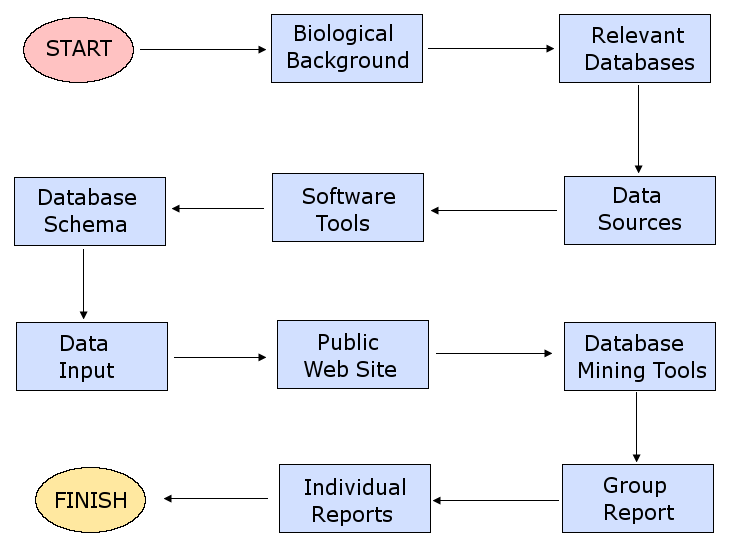
\includegraphics[scale=0.5]{pictures/workplan.png}
\caption{The work plan.}
\label{workplan}
\end{figure}

One of these steps was to locate all existing relevant databases that were available to the public and provided services similar to what we wanted to achieve.
Since the work of Cohen, who in 2002 estimated that the number of proteins which get phosphorylated can be up to 50 \cite{phosphorylation_origins}, a lot of research and experimenting has followed.
Several kinase, phosphatase and substrate databases have been published, such as Phospho.ELM \cite{phosphoELM}, Phosida \cite{PHOSIDA}, PhosphoPOINT \cite{PhosphoPoint} and networKIN \cite{networKIN}, which provide useful online resources for phosphoproteins across various species.
Protein post-translational modification by kinases and phosphatases is still an active area of research and therefore more data sources are constantly added to the list that was mentioned previously.
A thorough survey of these resources was essential in order to make sure that our work would not be redundant and that it would provide the maximum benefits to the users.
We reviewed them carefully and decided to use some of them as our primary data sources.
Since there were multiple sources of data, we had to choose only the ones that were most significant and that offered high quality data in a format that could be easily read and parsed by a computer.
All the data sources that we finally used are described in more detail in a subsequent chapter.

The next step involved choosing the software tools that we were going to use.
A plethora of tools were proposed by the group members and we had to carefully examine each one of them, list its advantages, disadvantages and capabilities
and finally decide on which ones to use.
At the end we chose to use the MySQL relational database management system and the Django web framework for creating the web interface in Python.
The reasons why we chose these tools, along with a brief description of each one of them, are provided in the next section.

After having a comprehensive list of all data sources and their details, we had to figure out ways of using them in order to map kinases and phosphatases to their corresponding substrates and find potential kinase-phosphatase pairs.
Moreover, we had to think about and analyze the requirements that any interested researcher would have from our database.
For this purpose we used the valuable advice of Prof. Michael Stumpf and Dr. Frances Turner.
Based on the above analysis and taking into careful consideration the advice of our project supervisor, we created the database schema to be used for KiPhoDB.
During the construction of any database, the development of the database schema is the single most important step, because it defines the nature of the information that can be stored to it.
Therefore we had to spend a lot of time and effort on deciding the form of KiPhoDB, its tables and their data fields. 
Moreover, as we started inputting real data into the database, we often had to update and improve the database schema so that it would reflect the nature of the data and the needs of the users.

Once we had finalized the database schema, we focused on the creation of the public web site and the insertion of more data in the database.
For this purpose, we created a logo for the project and all the web templates that were going to be displayed to the public user.
Subsequently we had to link these web templates with the database, so that they could draw information from it and present it to the users in a convenient and comprehensive format.
Furthermore, we also created and integrated into the website various software components that enabled users to search the data in the database, perform SQL queries that were sent directly to the MySQL server, browse the data, administer the database and the web site and visualize phylogenetic trees.
Automated scripts were also written in python, with the aim of keeping all database entries correct and up to date.
More details about the software tools and components that we implemented can be found in later chapters.


